\documentclass[11pt,a4paper]{article}
\usepackage{ls}
\usepackage[english]{babel}
\setlist{noitemsep}
\title{Systems, Organisations, Management}  

\author{Hans-Gert Gr\"abe}

\date{October 24, 2021}

\begin{document}
\maketitle

\section{Organisations as Systems}

Systematic innovation methodologies such as TRIZ are essentially based on a
better understanding of the development dynamics of corresponding (technical
and non-technical) \emph{systems}.  The results are rooted in engineering and
managerial experience from structured processes of planning, implementation
and operation of such systems. Increasingly, cooperative interdisciplinary
collaboration matters rather than the one brilliant mind that commands
thousand hands. The \emph{socio-technical character} of contradictions is
thereby intensified and opens up new dimensions of contradiction management.

This seminar topic aims to shed more light on the connection between the
concepts of system and (social) organisation. \textbf{Social organisations}
such as companies, associations, projects, unions, parties, governments,
states ... are undoubtedly theoretically delimitable and practically delimited
parts of reality with outwardly (and inwardly) directed goals and purposes
whose internal structure and dynamics are driven by an external throughput of
energy, material and information, and which can therefore be studied from a
systemic perspective.

The external throughput of energy, material and information is usually not in
the focus of consideration, as these throughputs are already mentally charged
in language form in a \textbf{more complex social context} and in the form of
interests, needs, monetary flows and power relations. Nevertheless, a systemic
structure is clearly recognisable, which is to be worked out in various
theoretical approaches that we will look at in more detail. In particular, the
concepts of \emph{action space} and \emph{cooperative action} in such spaces
will be conceptualised in more detail.

\section{Leadership and Management}

\emph{Management} is an essential form of influencing the dynamics and
development of organisations. Shchedrovitsky emphasises that one can only
manage something that is in motion\footnote{"Management is only possible if
  the object we manage is in motion, self-propulsion. Management is the use of
  this self-propulsion by managers for their own purposes." \cite[p. 28]{MSM}}
and that there is no need for management if there are no problems.

In the previous semester, we had already considered the topic by studying
different theoretical approaches to management.  Most of them assumed a
manager as a single leader and developed approaches and patterns of how
persons in such a \emph{role} can develop leadership in achieving given goals.
If we project such approaches onto a systemic concept of development in
contradictions, there seems to be a recurring central contradiction between
the goals of the organisation and the goals and interests of the people
involved in realising them.

However, such leadership principles have been under massive pressure for at
least 20 years, as they have only limited effect in modern contexts of action
in interdisciplinary teams. Even more, they presuppose the authorised
individual leader who combines management and leadership in one person. In
multi-stakeholder contexts such as socio-cultural or socio-ecological systems,
even this prerequisite is not given.

In this context, Shchedrovitsky clearly distinguishes between the notions of
\emph{management} and \emph{leadership} \cite[p. 27-30]{MSM} and shows to what
extent a new principal is confronted with contradictory challenges of both
concepts.

\section{Systemic Management Basics}

In the further course of the seminar we want to discuss the systemic
development of social organisations in the unity and difference of
\emph{planned action} and \emph{experienced results} in the light of different
theoretical approaches.

This requires a concept of \emph{action planning}, based on a \emph{conceptual
  understanding} of the process landscape within and around the organisation
in an appropriate explicit form of description and \emph{intelligible
  operational actions}.

The formulated intelligible actions -- the \emph{plan} -- is in
\emph{contradictory tension} with the processes actually taking place: On the
one hand, it has a controlling effect on these practices, on the other hand,
those practices partially resist this control.

This difference must be fed back to the planning process as an
\emph{evaluation of experienced results} in order to keep also the divergence
between plan and reality under control.

Relating planning and experience dimension is only possible on a language
level and requires a \emph{system of notions} to accompany the practical
real-world development by a discursive process (as \emph{practice of thinking}
in the unity and difference of \emph{pure thought} and \emph{mental activity}
as explained in \cite[p. 33-51]{MSM}).

This system of concepts is more stable than the real-world practices, but it
is not static -- it develops together with the practices.
\textbf{\emph{World} is \emph{reality for us} and thus reality in the process
  of conceptual grasping.}

These basic considerations are about \emph{processes} and \emph{procedures}
within an \emph{organisation}.

\section{Organisations}

What is an organisation? Wikipedia distinguises between formal aud informal
organisations. 

\paragraph{Formal organisations.}
\begin{quote}
  An organisation that is established as a \emph{means for achieving defined
    objectives} has been referred to as a formal organisation. Its design
  specifies how \emph{goals are subdivided and reflected} in subdivisions of
  the organisation. Divisions, departments, sections, positions, jobs, and
  tasks make up this work structure. Thus, the formal organisation is expected
  to \emph{behave impersonally} in regard to relationships with clients or
  with its members. [...] A \emph{bureaucratic structure} forms the basis for
  the appointment of heads or chiefs of administrative subdivisions in the
  organisation and endows them with the authority attached to their position.
  (Wikipedia, my emphasis)
\end{quote}
See about the "impersonality" and also the "automaton" in the quote by Marx in
my first lecture.

\paragraph{Informal organisations.}
\begin{quote}
  [...] The informal organisation expresses the personal objectives and goals
  of the individual membership. Their objectives and goals may or may not
  coincide with those of the formal organisation. [...] (Wikipedia)
\end{quote}
The further explanations in Wikipedia remain weak and contradictory.
Structure-building processes and especially shared conceptual systems also
develop in informal organisations, with exciting new structuring processes
of co-operative action taking place that are of particular interest to us in
the seminar. Wikipedia is a reflection of the weakness of the conceptual basis
in this field.

Also ORG -- the \emph{organisation ontology of the W3C} \cite{vocab-org} --
considers \texttt{org:OrganisationalUnit}, \texttt{org:FormalOrganization} and
\texttt{org:OrganizationalCollaboration} as subconcepts of the concept
\texttt{org:Organization} but does not mention informal organisations.  In
their definition an organisation
\begin{quote}
  represents a collection of people organized together into a community or
  other social, commercial or political structure. The group has some common
  purpose or reason for existence which goes beyond the set of people
  belonging to it and can act as an Agent. Organisations are often
  decomposable into hierarchical structures.~\cite{vocab-org}
\end{quote}

\texttt{org:Organization} is related to \texttt{foaf:Agent}, 
\begin{quote}\raggedright
  ... the class of agents; things that do stuff. A well known sub-class is
  \texttt{foaf:Person}, representing people. Other kinds of agents include
  \texttt{foaf:Organization} and \texttt{foaf:Group}. \cite{foaf}
\end{quote}

A \texttt{foaf:Group}
\begin{quote}
  ... represents a collection of individual agents (and may itself play the
  role of a Agent, i.e. something that can perform actions).

  This concept is intentionally quite broad, covering informal and ad-hoc
  groups, long-lived communities, organisational groups within a workplace,
  etc. ...
  
  While a Group has the characteristics of a Agent, it is also associated with
  a number of other Agents (typically people) who constitute the Group, its
  members. ...  The basic mechanism for saying that someone is to use the
  member property of the Group to indicate the agents that are members of the
  group.
\end{quote}
The terms Agent and Group thus introduce self-similar concepts of structures
that are \emph{capable of action}. This corresponds to the legal construction
of a \emph{juridical subject} (juristisches Subjekt) in the sense of the Civil
Code (BGB) if \emph{responsibility for the consequences of action} is added.

\section{Organisations as Socio-Technical Systems}

While in the Wikipedia definition positions, jobs and tasks are mentioned, but
beyond bureaucracy no people, in this definition an organisation is a
"community of people". However, it has a goal that does not result from the
set of goals of the people involved, but is an emergent function of the
organisation -- the whole is more than the sum of its parts in the sense that
relational synergy effects are of special importance in such an organisation.

This corresponds closely with the \emph{system concept} developed so far:
\begin{quote}
  A \emph{system} is a \emph{delimited set of elements} (components, objects,
  resources) that are interconnected and interact with each other. Their
  interaction realises a \emph{qualitatively new function} (emergent function)
  and thus constitutes a \emph{new unified whole}.

  A system has a \emph{structural} and an \emph{operational} dimension which
  are in contradictory dialectical relation of decomposability and
  indecomposability.

  The \emph{operation of a system} requires a qualitatively and quantitatively
  defined throughput of energy, material and information.
\end{quote}

Ian Sommerville \cite{Sommerville2015} also starts with the concept of a
system and moves from there to the concept of \emph{organisation}.
\begin{quote}
  A system is a meaningful set of interconnected components that work together
  to achieve a specific goal.  \cite{Sommerville2015}
\end{quote}
Right after that comes a distinction between technical and socio-technical
systems:

\paragraph{Technical computer-based systems}
are systems that contain hardware and software components, but not procedures
and processes. ... Individuals and organisations use technical systems for
specific purposes, but knowledge of that purpose is not part of the system.
For example, the word processor I use does not know that I am using it to
write a book.

\paragraph{Socio-technical systems}
contain one or more technical systems, but beyond that -- and this is crucial
-- the knowledge of how the system should be used to achieve a broader
purpose.  This means that these systems have \emph{defined work processes},
\emph{human operators} as integral part of the system, are \emph{governed by
  organisational policies} and are \emph{affected by external constraints}
such as national laws and regulations.

Essential characteristics of socio-technical systems:
\begin{enumerate}
\item They have special properties that affect the system as a whole, and are
  not related to individual parts of the system. These special properties
  depend on the system components and the relationships between them. Because
  of this complexity, the system-specific properties can only be evaluated
  when the system is composed.
\item They are often not deterministic. The behaviour of the system depends on
  the human operators and on other people who do not always react in the same
  way. Also, the operation of the system can change the system itself.
\item The extent to which the system supports organisational goals depends not
  only on the system itself. It also depends on the \emph{stability of the
    goals}, the relationships and \emph{conflicts between organisational
    goals}, and how people in the organisation \emph{interpret those goals}.
\end{enumerate}

In this context, there is a clear shift on the scale of controllability from
direct control (technical systems) to indirect control (socio-technical
systems), which in \textbf{socio-economic systems} with a large number of
stakeholders or even \textbf{socio-ecological systems} shifts further in the
direction of movement according to intrinsic laws ("natural processes").

This relates to TRIZ principle 25 \emph{Exploit Self-Service Processes}, which
counts as the mastery of engineering.  It claims that the best solution of a
task is reached if the aspired goals are realised "by themselves".

Ultimately, this means to resolve the contradiction between plan and
realisation and to develop a form of description that brings the "natural"
movement in a system according to its own laws in coherence with the human
goals and needs.

\section{Shchedrovitsky on Organisations}

What is an organisation for Shchedrovitsky? In \cite[p. 30 ff]{MSM} he
distinguishes three dimensions of that notion
\begin{itemize}
\item Organisational work
\item Organisation as the result and means of organisational work
\item Organisation as a form of life of the collective
\end{itemize}

\paragraph{Organisational work.}
\cite[p. 26]{MSM} When we organise we collect something. Let us take a look at
design. We need some structural elements, so there is a designer with a set of
elements. We must collect these elements in a particular way, and we must
establish some kind of connection and relations between them. When we are
doing this sort of work we must impose some organisational form on these
elements. [\ldots]

And when we have done such work on the integration of the elements and the
establishment between them of certain relations and connections, we stop this
work, and then the whole, which we have organised, can begin to operate
according to its laws. But its action according to its laws no longer belongs
to organisational work.

Organisers deal with a particular set of elements, collect elements of a
certain type and form in particular quantities, combine them and set certain
relations and connections between them. When they have done this and have thus
created the structure of the organisation – and the structure is defined by
the location of the elements and the type of connections and relations – they
recede into the background, and this thing either remains dead or begins to
operate according to its laws.

\paragraph{Organisation as the result and means of organisational work.}
\cite[p. 29]{MSM} Organisation as the result of organisational work can be
regarded as both an \textbf{artificial entity} and as \textbf{naturally living
  thing}.

Who takes an artificial view of organisations? Organisers themselves. And
those who design and create organisations always look at them as their own
creations.  The organiser makes it, and in this sense organisations can be of
any kind depending on the goals and objectives of the organiser. The main
question is: why does the organiser create a particular organisation?
[\ldots]

The organisation acts here as an \textbf{artificial entity}. It has a purpose
(Zweck) and can be considered, as can any structure, in terms of the functions
that it, the organisation, must provide. So we are talking about the functions
of the organisation, about the purpose of the organisation.  These are all
characteristics that are seen from an artificial point of view.

As a tool, as a means, \textbf{as an artificial entity, the organisation does
  not and cannot have goals} (Ziele). Organisers can have goals. But for their
goals, in relation to their goals, the organisations they create are a means,
a means for them to achieve their goals.

\paragraph{Organisation as a form of life of the collective.}
\cite[p. 30]{MSM} The organisation has been created. And the organiser – a
pure organiser, not a manager – has gone. The organisation has been created,
and it has begun to live its own life. And then it turns out that, from a
natural point of view, other goals may appear in this organisation – the goals
of the collective, which was organised. Generally, something quite different
begins, this \textbf{organisation begins to live its own life}. Then we
[\ldots] must seek forms, methods, laws of the life of the groups and the
collectives within organisations.

When the organisation is seen from a natural viewpoint, it is not yet the
means, but the \textbf{form}, the \textbf{condition} of the life of the
collective (the people) who work in it.

And it is even possible to see the organisation in the same way as we see the
sunrise and sunset: the people working in it completely forget that the
organisation was created by some other person to resolve particular
objectives, achieve particular goals, for a particular purpose. It, this
organisation, will be perceived by them like the movement of the heavenly
bodies, as a natural condition of life.

\section{Systematic Management in Organisations}

The subject of \emph{systematic management} are socio-technical and especially
socio-economic systems. The latter consist of economic units (companies,
government, state, ... ) that are interconnected in a market-like manner. The
\emph{world of economic units} has a systemic structure similar to the world
of technical systems.

In the understanding developed above, \textbf{management} therefore means to
\emph{control} the processes taking place in the (living) organisation with
the \emph{goal} to implement the \emph{purposes} of the organisation in an
efficient way.

This is necessary to be operated on several spatio-temporal levels (micro and
macro processes), whereby short term goals and long term goals are in 
contradictory tension. Therefore, management is usually divided into several
relatively autonomous levels
\begin{itemize}
\item Strategic management
\item Middle management
\item Operational management
\item Infrastructure management and support
\end{itemize}
which are themselves in systemic system-subsystem interrelations and thus in a
co-evolutio\-nary relationship which is best processed via a control loop
designed as a feedback loop.

\subsection{Systematic Management and ISO 9000}

Systematic management requires a descriptive approach to this control loop as
part of the organisation's process model, such as given in the modified
process model of ISO 9000:2008.
\begin{center}
  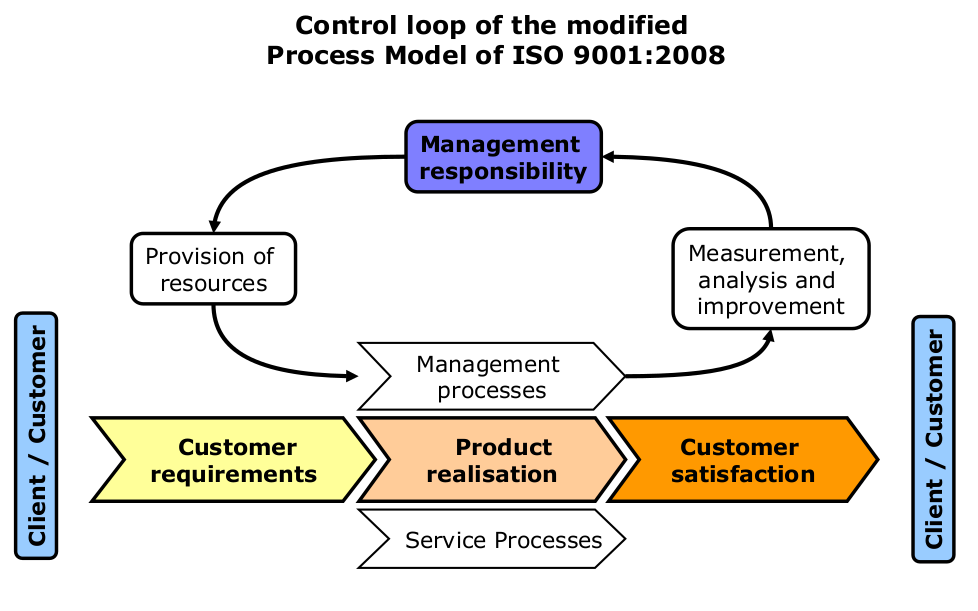
\includegraphics[width=.8\textwidth]{2.png}\\ \textbf{Fig. 1:} Control Loop
  in the Modified Process Model of ISO 9000
\end{center}
ISO 9000 is a set of general quality assurance standards to \textbf{assess}
the process quality of enterprises. It is a descriptive standard and not
directed towards improvement of process quality (although can be used for such
an improvement in combination with other tools).
\begin {itemize} 
\item It is mainly a European standard.
\item It is used mainly to assess the process quality of suppliers that
  demonstrate with a ISO 9000 certificate their ability to produce in a
  negotiated frame of time, costs and performance. 
\item Set of standards for the proof of process quality for the creation as of
  material so also of intangible products and services.
\item Framework with a lot of leeway for corporate strategy and concrete
  management goals.

  Minimum requirements for a QM system according to ISO 9000: complete,
  documented, known, verifiable, evolutionary
\end {itemize}
ISO 9000 contains minimum requirements for the structural and procedural
organization, so that quality is not a coincidence, but the result of a
controlled process.

Note that the process model shown in fig. 1 is a \emph{standard model} at a
higher language level (\textbf{meta-model}) than the respective process models
of the individual organisations, but unlike the process model of a real-world
organisation, it has no real-world instantiation. Such a phenomenon is well
known in computer science in connection with abstract classes.

Fig. 2 shows the relation between the ISO norm, quality management documents
and real-world process quality at three different levels within a company.  

\begin{center}
  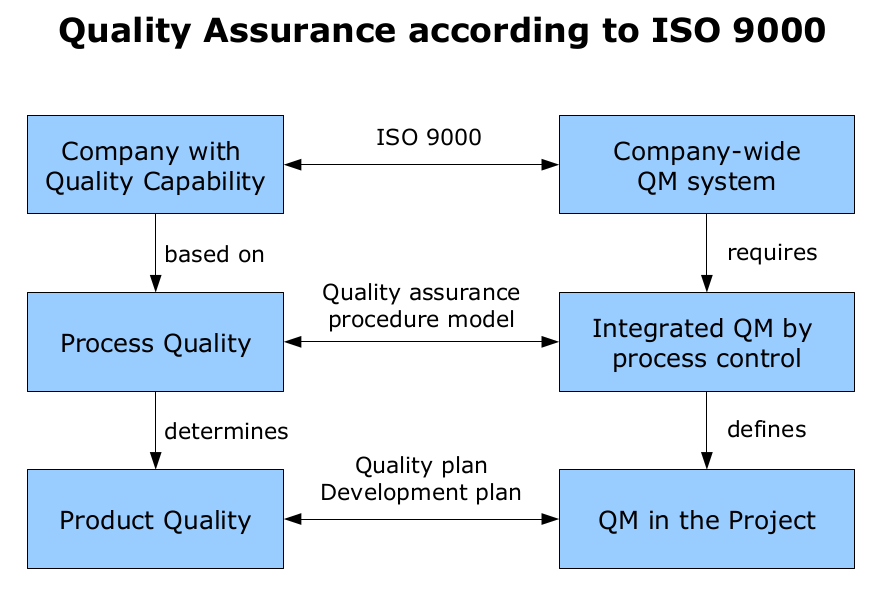
\includegraphics[width=.8\textwidth]{1.png}\\ \textbf{Fig. 2:} The relation
  between model, meta-model and meta-meta-model in quality assurance
\end{center}

\subsection{Managing Organisational Development and\\ Capability-Maturity
  Models} 

Management is only possible in the context of a clear understanding of the
structural and procedural organisation of the organisation.  In order to
capture this in descriptive terms, a \textbf{separation of functions and
  resources} is necessary. In particular, "human resources" are removed from
the description and replaced by the term \textbf{role}.

In this way, a \emph{functional decoupling from the resources} is achieved at
design time -- only at runtime this position must be connected "just in time"
with a qualified resource that was produced beyond the horizon of the concrete
planning processes.

Only with such a decoupling (and only at the level of such a decoupling) it is
possible as management to take an external standpoint on its own activities.
Only in this way is \textbf{structurally driven organisational development}
possible. There are other culturally driven approaches such as TQM, which will
be discussed separately (the Toyota model).

Systematic management through structurally driven organisational development
means above all the creation and improvement of conditions for the management
of well-structured processes.

CMMI (Capability Maturity Model and its predecessor CMM) is such a process
model for organisations such as software companies that are project-driven and
do not have a continuous production process. The model is a \textbf{maturity
  model} and supports such companies to introduce and improve a company-wide,
uniformly structured project management
\begin{itemize} 
\item from the structuring of individual projects into \emph{process
  activities and milestones}
\item through the definition of \emph{company-wide uniform or specifically
  adaptable process modules}
\item and the \emph{uniform quantitative measurement} of such building blocks
\item to the introduction of \emph{qualified error and change management}.
\end{itemize}
\begin{center}
  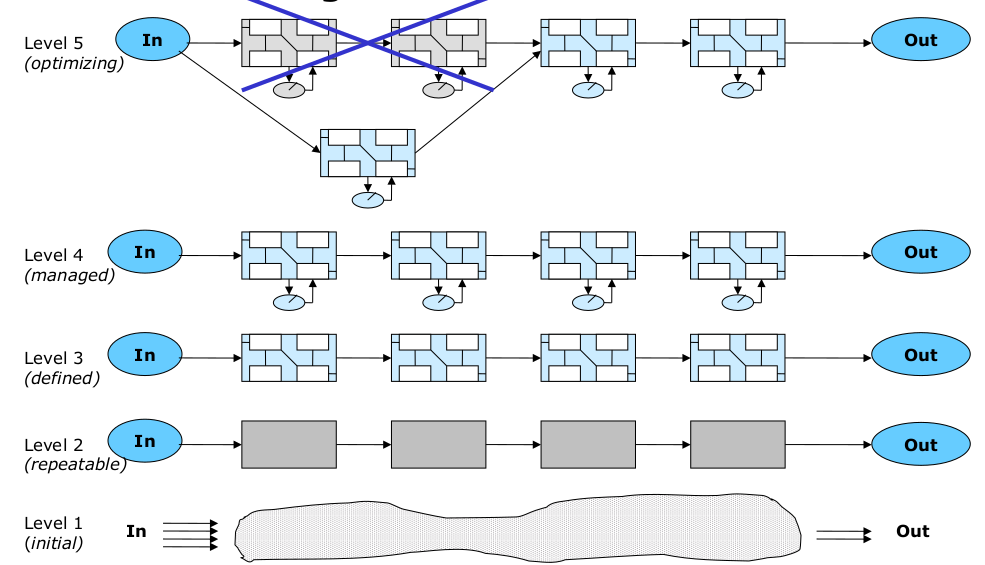
\includegraphics[width=.8\textwidth]{6.png}\\ \textbf{Fig. 3:} Increasing
  maturity of structured project management within CMM(I)
\end{center}
These four transitions are assigned five maturity levels. The transitions are
supported by concentrating on predefined \emph{key process areas} and
\emph{key practices}.

\subsection{Additional Reading: CMMI in More Detail}

\subsubsection{The Maturity Levels}

The five maturity levels according to which processes of an organization are
evaluated.

\paragraph {Initial Process}
\begin {itemize} 
\item Process exists only informally
\item Low adherence to deadlines and costs, high risk
\item Chaos, "heroism", fire-fighting operations
\end {itemize}

\paragraph {Repeatable Process (CMMI: Managed)}
\begin {itemize} 
\item There are defined and structured requirements for the process
\item "Learn from similar projects" (requirements management, project
  management and quality management)
\end {itemize}

\paragraph {Defined Process}
\begin {itemize} 
\item Procedures and individual process activities are clearly defined
\item The organization is in the learning focus
\item Process definition, training programs, team coordination
\end {itemize}

\paragraph {Managed Process (CMMI: Quantitatively Managed)}
\begin {itemize} 
\item Central control that systematically collects process measures
\item Process and product development are quantitatively analyzed and rated
\item Information is used as support for decision-making 
\end {itemize}

\paragraph {Optimizing Process}
\begin {itemize} 
\item "Self-dynamically optimizing process" 
\item Process measures are systematically used for dynamic process control and
  monitoring
\item Process change management
\item Technology change management
\end {itemize}

\subsubsection{Expectations}
The higher the level of maturity, 
\begin {itemize} 
\item the more precisely goals are achieved.
\item the less is the difference between the target and actual results.
  \begin {itemize} 
  \item Level 1 companies miss their deadlines at large. 
  \end {itemize}
\item The fluctuation range of the actual values around the target
  specifications is lower.
  \begin {itemize} 
  \item Similar projects are completed within a narrower time frame.
  \end {itemize}
\item Costs and development time decrease, productivity and quality increase.
  \begin {itemize} 
  \item Higher process efficiency, low rework rate.
  \end {itemize}
\item Expectations are more likely fulfilled in standard projects.
\item But: New techniques and applications are reducing the process capability
  due to higher variability.
\end {itemize}

\subsubsection{Determination of the Maturity Level according to CMM}

For each stage a number of \textbf {Key Process Areas} are defined in which an
organization of this level has to reposition itself implementing appropriate
given \textbf {Key Practices}.

\subsubsection*{Level 1: Initial Process}
\begin {itemize} 
\item No criteria and specifications
\item Project and quality management may or may not exist but are not 
  consistently applied.
\item Projects are managed at short notice, adaptively and reactively.
\end {itemize}

\subsubsection*{Level 2: Repeatable (CMMI: managed) Process}

\emph {Goal:} Introduction of a basic project monitoring and management,
planning and control.
  
\emph {Focus:} Leadership principles, structure and management of projects.

\emph {Key Process Areas and Key Practices:}
\begin {itemize} 
\item \textbf {Requirements management}
  \begin {itemize} 
  \item Establish a common understanding between customer and project team
    about the requirements.
  \end {itemize}
\item \textbf {Project planning, tracking and monitoring}
  \begin {itemize} 
  \item Transparent presentation of the development progress in order to be
    able to initiate correction measures at early stage.
  \end {itemize}
\item \textbf {Sub-order management}
  \begin {itemize} 
  \item Select, control and monitor qualified sub-suppliers.
  \end {itemize}
\item \textbf {Quality management} on process and product level, configuration
  management
  \begin {itemize} 
  \item Ensure integrity of the products throughout their entire life cycle.
  \end {itemize}
\end {itemize}

\emph{Result:}
\begin {itemize} 
\item Processes as a sequence of "black boxes" with milestones as checkpoints.
\item Stable project management.
\item Processes can be predicted within limits through constant monitoring.
\item Cross-project experience can be quantified.
\end {itemize}

\subsubsection*{Level 3: Defined Process}

\emph{Goal:} Definition and introduction of an organization-wide valid unified
software process; internal structure of the phases is defined and
understanding of roles is visible.

\emph {Prerequisite:} Projects are planned, managed and monitored (level 2) as
a sequence of processes according to uniform principles.

\emph {Focus:} Process descriptions.

\emph {Key Process Areas and Key Practices:} Focus on process organization
\begin {itemize} 
\item \textbf {Definition} of processes
  \begin {itemize} 
  \item Development and maintenance of a useful set of process values.
  \end {itemize}
\item \textbf {Training program}
  \begin {itemize} 
  \item An independent unit is responsible for employees' training.
  \end {itemize}
\item \textbf {Coordination} between project teams (exchange of experience)
\item \textbf {Integrated SW Management}
  \begin {itemize} 
  \item Development and management are integrated into one over the entire
    life cycle defined process.
  \item Standard processes can be tailored to projects.
  \end {itemize}
\item \textbf {SW Product engineering}
  \begin {itemize} 
  \item Process integrates all technical activities to ensure to produce
    correct, consistent products effectively and efficiently.
  \end {itemize}
\end {itemize}

CMMI further subdivides some of the main process areas
\begin {itemize} 
\item \textbf {Coordination}
  \begin {itemize} 
  \item Integrated team building
  \item Integrated sub-order management
  \item Decision analysis
  \item Integration organization infrastructure
  \end {itemize}
\item \textbf {Integrated SW Management}
  \begin {itemize} 
  \item Integrated project management
  \item Risk management
  \end {itemize}
\item \textbf {SW Product Engineering}
  \begin {itemize} 
  \item Requirements analysis
  \item Technical solution
  \item Product integration
  \item Verification
  \item Validation
  \end {itemize}
\end {itemize}

\emph{Result:} Improved, describable quality; institutionalised process
prototypes that are maintained and further developed.

\subsubsection*{Level 4: Managed (CMMI: Quantitatively Managed) Process}

\emph{Objective:} Quantitative measurement of the quality of products and the
productivity of processes through an organisation-wide metrics programme as an
objective basis for decision making.

\emph{Prerequisite:} Uniform understanding across the organisation about
projects and process models (level 3) and active project management (level 2).

\emph{Focus:} Process measurement.

\emph{Key Process Areas and Key Practices:}
\begin{itemize}
\item \textbf{Quantitative process management}
  \begin{itemize}
  \item Quantitatively control and monitor process performance.
  \end{itemize}
\item \textbf{Quantitative quality managament}
  \begin{itemize}
  \item  Develop quantitative understanding of product quality.
  \end{itemize}
\end{itemize}

CMMI clarifies as follows:
\begin{itemize}
\item Quantitative project management
\item Performance of organisational processes
\end{itemize}

\emph{Result:} Time, cost and quality become fairly predictable.

\subsubsection*{Level 5: Optimising Process}

\emph{Objective:} Introduction of a continuous and measurable process for
improvement of software development.

\emph{Prerequisite:} Quantitative monitoring information (level 4) and
application of innovative ideas and technologies.

\emph{Focus:} Process alignment.

\emph{Key Process Areas and Key Practices:}
\begin{itemize}
\item \textbf{Error avoidance}
  \begin{itemize}
  \item Identify and eliminate causes of errors.
  \end{itemize}
\textbf{Product innovation management}
  \begin{itemize}
  \item Integration of new technological developments at product level.  
  \end{itemize}
\textbf{Process innovation management}
  \begin{itemize}
  \item Identification of new, useful ideas and their orderly introduction.
  \end{itemize}
\end{itemize}
CMMI specified:
\begin{itemize}
\item Organisation-wide introduction of innovations
\item Analysis of causes and elimination of errors
\end{itemize}



\begin{thebibliography}{xxx}

\bibitem{foaf} FOAF Vocabulary Specification (2014).\\ W3C Recommendation.
  \url{http://xmlns.com/foaf/spec/}.
\bibitem{vocab-org} The Organization Ontology (2014).\\  W3C Recommendation.
  \url{https://www.w3.org/TR/vocab-org}.
\bibitem{Sommerville2015} Ian Sommerville (2015). Software Engineering.
  Chapter 19 „Systems Engineering“.

  Slide stack available at Sildeshare\\{\small
  \url{https://www.slideshare.net/software-engineering-book/ch19-systems-engineering}}

\bibitem{MSM} Georgy P. Shchedrovitsky.  Selected Works. A Guide to the
  Methodology of Organisation, Leadership and Management. Part I in
  Khristenko, Reus, Zinchenko et al.  Methodological School of Management.
  Bloomsbury Publishing 2014.  ISBN 978-1-4729-1029-5.
\end{thebibliography}

\end{document}

